% !Mode:: "TeX:UTF-8"
\documentclass[master,openright,twoside,a4paper,AutoFakeBold]{sudathesis}

% == 内置的package ==
% 添加pdf文件 includepdf命令
\usepackage{pdfpages}
% 全局修改cite为右上角方括号 ；如果使用Overleaf可以注释掉下面2行，使用\upcite() (无自动补全)
\usepackage{natbib}
\setcitestyle{super, square, sort&compress}
% algorithm环境
\usepackage[ruled,linesnumbered]{algorithm2e}
\renewcommand{\algorithmcfname}{算法} % caption部分显示中文名“算法”
% == =========== ==

% == 按需要导入你自己的package ==
\usepackage{graphicx}
\usepackage{float}          % 图表强制位置H
\usepackage{multirow}   % 表格合并单元格
\usepackage{booktabs}  % 表格用于创建漂亮的水平线
\usepackage{stfloats}     % 跨栏图片*/表格*美化
\usepackage{pifont}        % 勾叉符号
\usepackage[skins]{tcolorbox}  % 文本框
\tcbuselibrary{breakable}% 支持文本框跨页
\usepackage{boites, boites_exemples}
\usepackage{amsmath}

\newif\iffinalversion
% 设置为送审版
% \finalversionfalse
% 设置为最终版
\finalversiontrue

% 论文相关信息
\school
{计算机科学与技术学院}{School of Computer Science and Technology}

% 专业中英文名
\major
{人工智能}{Artificial Intelligence}

% 学位类型，学术/专业
\degreetype
{专业}

% 方向中英文名
\direct
{代码生成}{Code Generation}

% 论文中英文标题
\thesistitle
{XXX代码生成方法研究}{XXX Code Generation Methods}

% 论文封面中文标题，若只需一行则第二行留空{}
\coverthesistitlech
{XXX代码生成方法研究}
{}

% 论文封面英文标题，若只需一行则第二行留空{}
\coverthesistitleeng
{XXX Code Generation Methods}
{with Large Language Models}

% 作者中英文名
\thesisauthor
{作者}{Author}

% 导师中英文名
\teacher
{导师}{Advisor}

% 导师职称
\teacherdegree
{教授}{Professor}

% 副导师中英文名，如无副导师则留空，否则指定\twoteacher后填写
% \twoteacher
\subteacher
{}{}

% 副导师职称
\subteacherdegree
{}{}

% 班级
\class{自然语言处理1班}

% 学号
\studentID{20235227XXX}

% 单位代码
\unicode{10285}

% 论文时间，用于首页
\thesisdate{2026}{6}

\begin{document}

\iffinalversion
    % 最终版通过导入pdf文件来生成封面
    
\includepdf[pages=-]{pdf/封面.pdf}
    \includepdf[pages=-]{pdf/blank.pdf}
    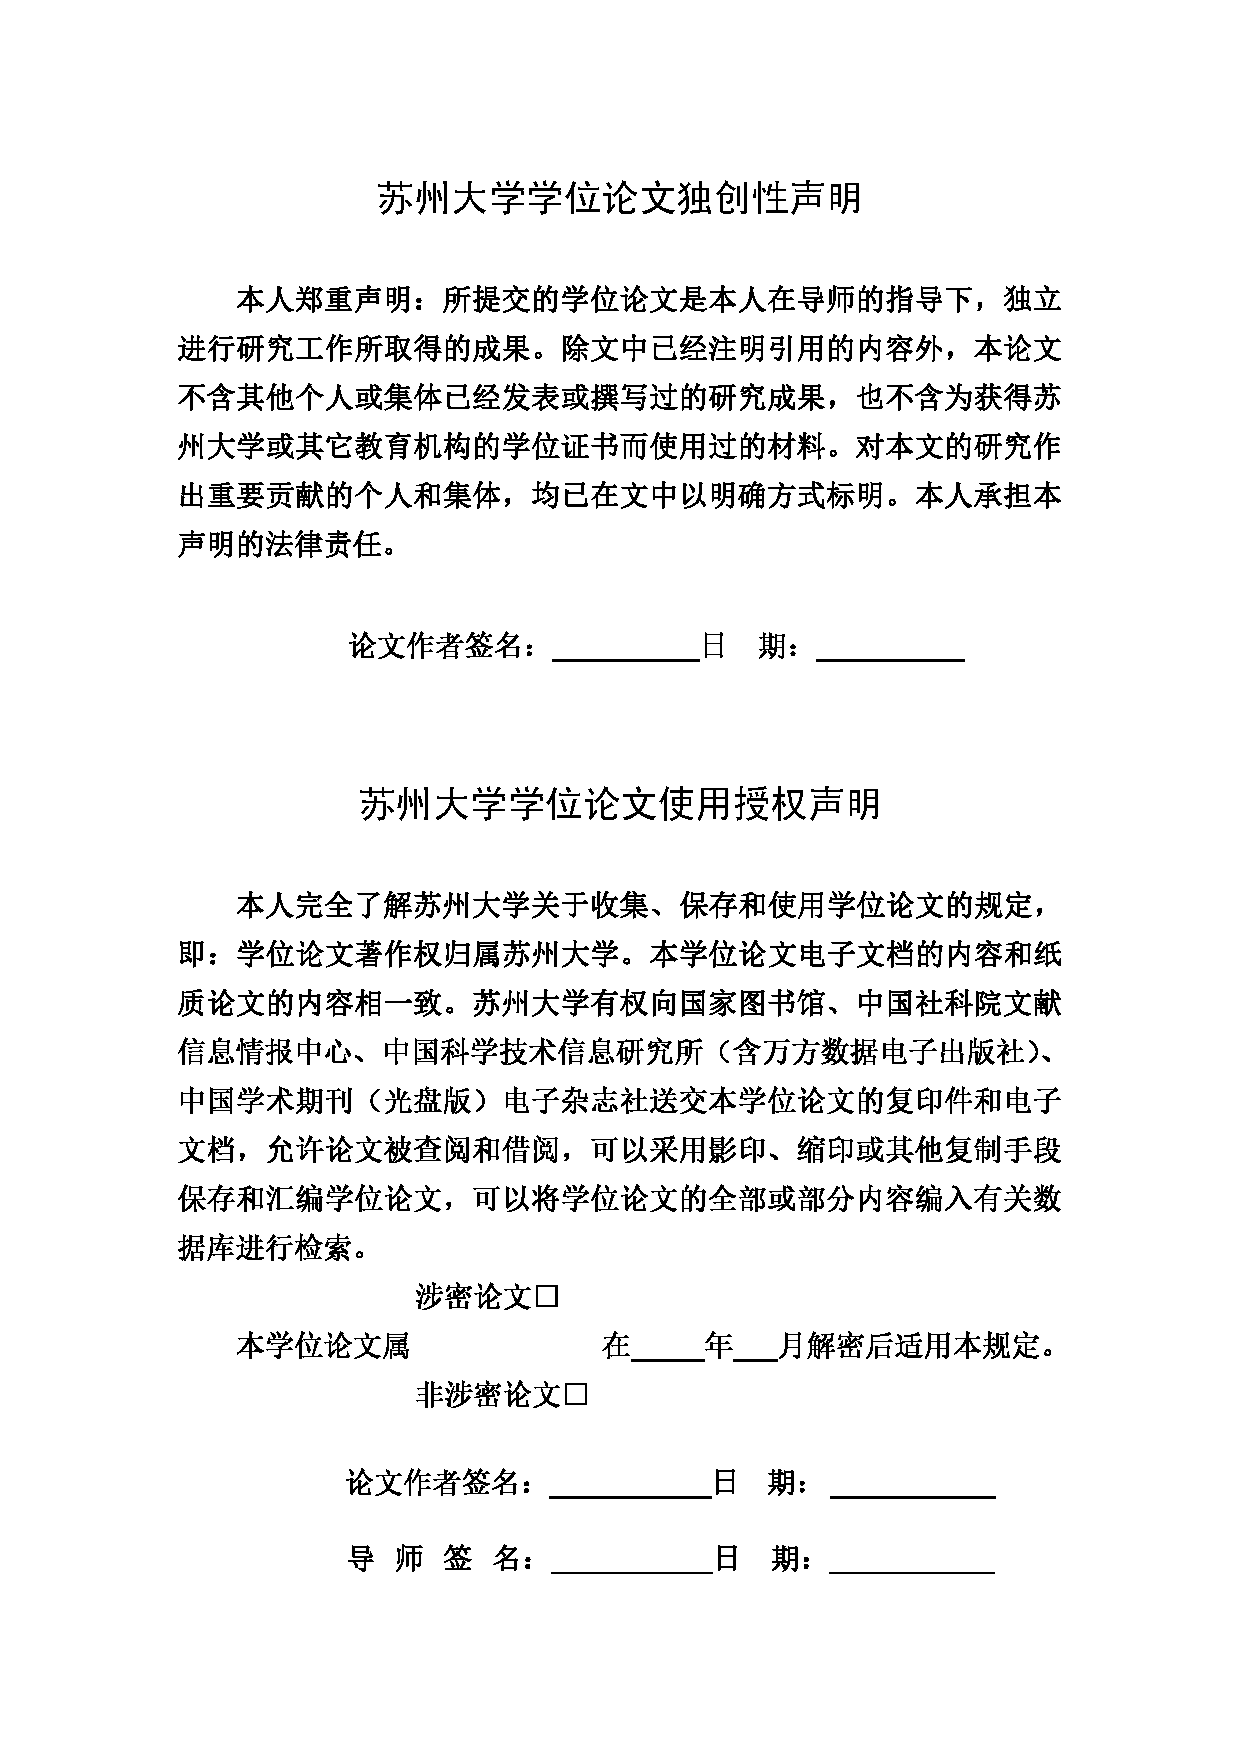
\includepdf[pages=-]{pdf/学位论文使用授权声明.pdf}
    \includepdf[pages=-]{pdf/blank.pdf}
\else
    % 送审版
    % 送审版通过导入pdf文件来生成封面
    
\includepdf[pages=-]{pdf/送审封面.pdf}
\fi

% 【摘要】
% 正文前页码是大写罗马字母
\pagenumbering{Roman}
% 前言页眉页脚样式
\pagestyle{cnfrontmatter}
\include{content/0_1_abstract-zh}

\pagestyle{enfrontmatter}
\include{content/0_2_abstract-en}

% 【目录】不设置页眉和页码
\makeatletter
\let \asas \ps@plain
\let \ps@plain \ps@empty
\makeatother
\pagestyle{empty}

% 生成目录
\tableofcontents
\setcounter{secnumdepth}{4}

\makeatletter
\let \ps@plain \asas
\let\asas\relax
\makeatother
\clearpage  %目录3页以上，使用cleardoublepage

% 正文页码样式
\mainmatter
% 正文页眉页脚样式
\pagestyle{mainmatter}
% 正文页码是阿拉伯数字
\pagenumbering{arabic}

% === 关闭正文章节强制奇数页开头的限制 ===
\makeatletter
\@openrightfalse
\makeatother
% ================================================

% 【正文】

\include{content/1_introduction}
\include{content/2_chapter}
\include{content/3_chapter}
\include{content/4_chapter}
\include{content/5_conclusion}

% % 参考文献,4或者小4楷体
\include{content/reference}

% % 附录,4或者小4楷体
% \appendix

% 附页标题样式
\backmatter

% 附页
\iffinalversion
    % 最终版
    % 最终版添加发表刊物和致谢
    % 附页
    \clearpage
\phantomsection
\chapter*{攻读学位期间的成果}
\markboth{攻读学位期间的成果}{}
\addcontentsline{toc}{chapter}{攻读学位期间的成果}

\begin{itemize}
	\setlength{\parsep}{2em}
	\item \textbf{\heiti\sihao{论文}}
	      \begin{enumerate}
		      \item \textbf{First Author}, Author. \emph{Paper Title}. Conference 2026.
	      \end{enumerate}

	\item \textbf{\heiti\sihao{软件著作权}}
	      \begin{enumerate}
		      \item XXX系统V1.0（登记号：2026SR*******，2026）
	      \end{enumerate}

	\item \textbf{\heiti\sihao{实习}}
	      \begin{enumerate}
		      \item XX科技有限公司，XX工程师，XXXX年X月至XXXX年X月
	      \end{enumerate}

\end{itemize}

    \clearpage
\phantomsection
\chapter*{致谢}
\markboth{致谢}{}
\addcontentsline{toc}{chapter}{致谢}

    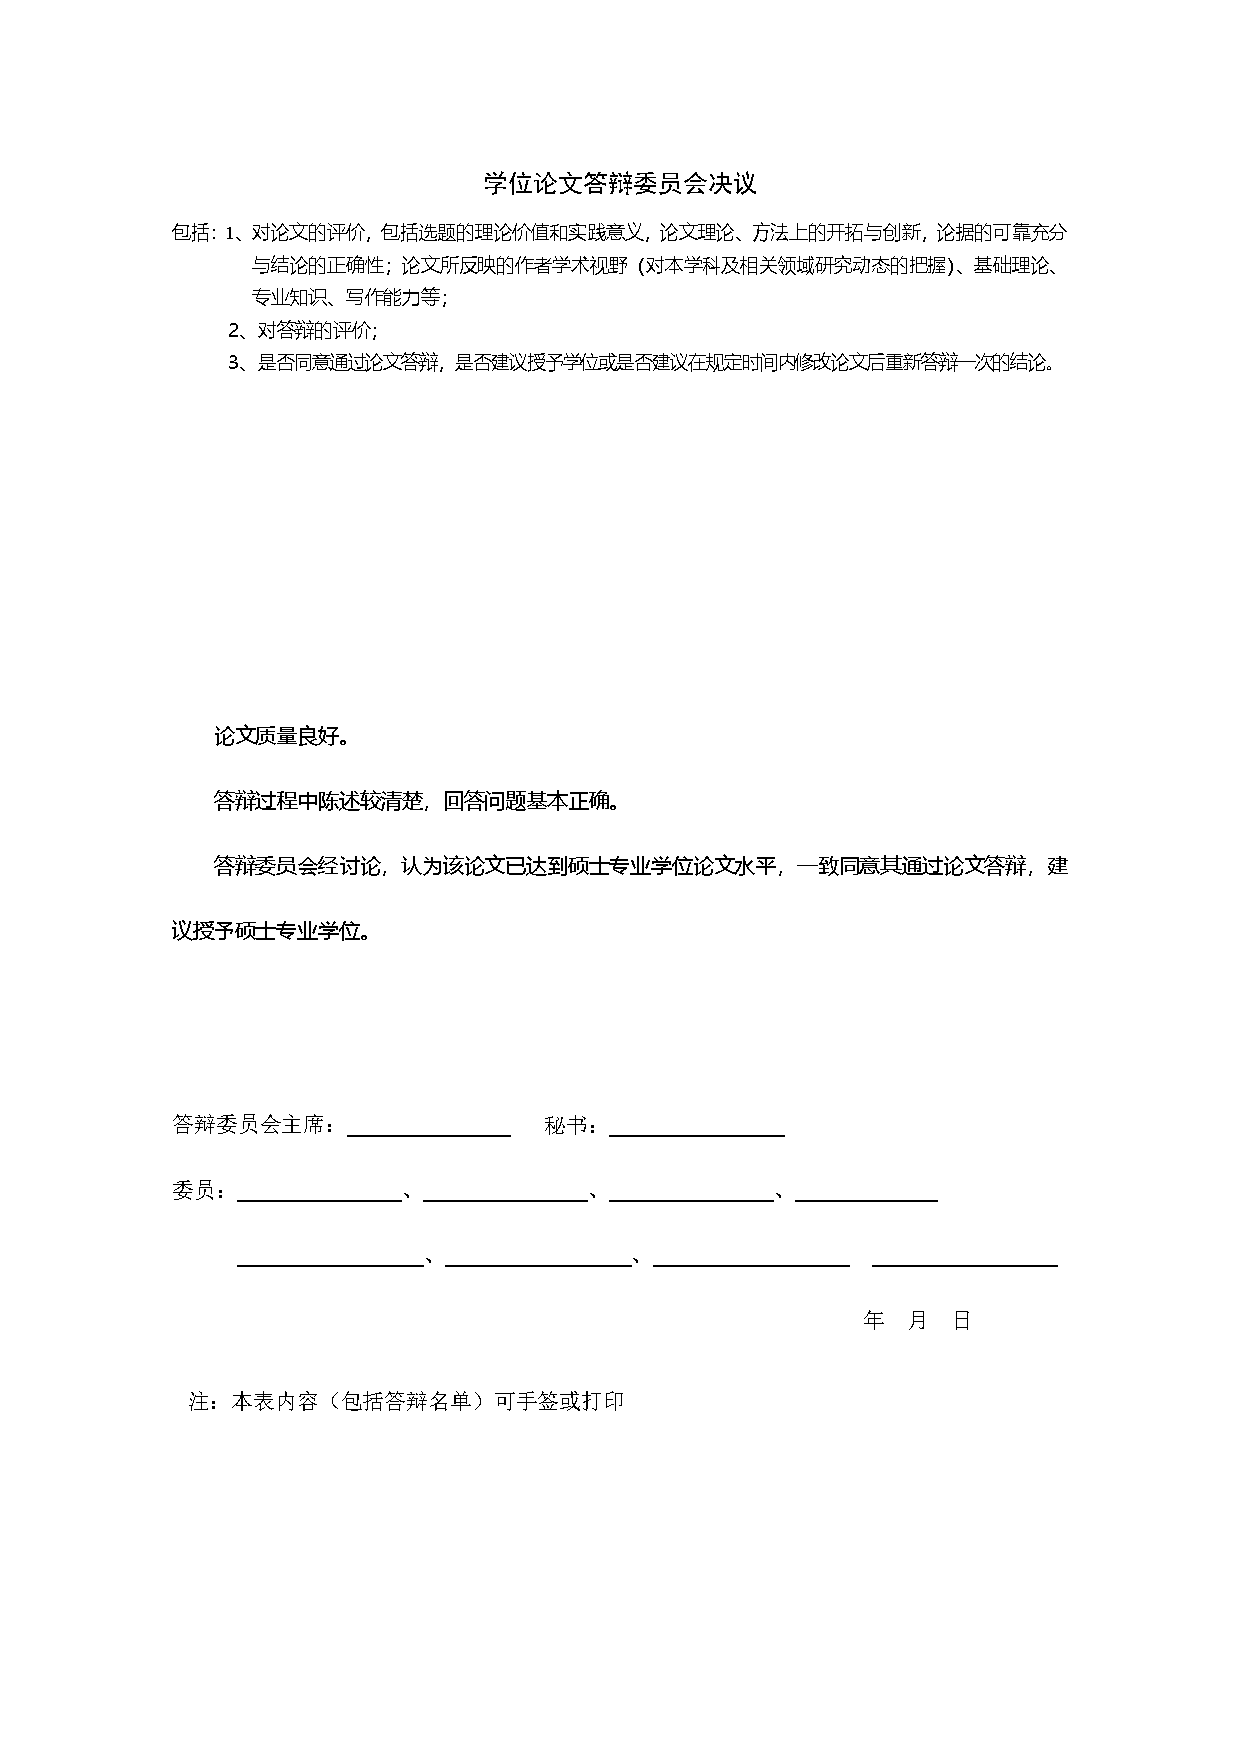
\includepdf[pages=-]{pdf/答辩决议书.pdf}
\else
    % 送审版
\fi

\end{document}